\chapter{Evaluation of Results}
\label{ch:results-evaluation}

\section{Methodology}
In order to evaluate the proposed solutions to the two questions posed in \cref{ch:intro},
the following methodologies has been used.

\begin{enumerate}
    \item To evaluate how error detection has been improved, compare the number of actual errors found
    in a form by the tools detected and against the proposed solution.
    
    \item To evaluate how the error information system has been improved, the number of elements that
    make up the error messages of each existing tool and of our solution is compared. In addition,
    a survey is carried out on different users familiar with the existing tools.

    \item To evaluate to what extent we can translate shapes to domain object models we collect all the
    existing shapes in GitHub, reduce the set to those that fit the micro compact syntax and try to
    generate objects for those that are syntactically and semantically valid. In this way we can
    approximate what percentage we can translate.
\end{enumerate}

\section{Datasets}
To test the above methodologies we will use two types of datasets.
real and synthetic. In the case of the real ones, as we do not know
any shape dataset, we will use the Big Query Google service to download
all the files with an open source license and extension \texttt{.shex}
that exist as of March 17, 2019 on GitHub. In the case of synthetic tests,
schemes are designed that contain the errors described, taking into account
the previous work.

\section{Results}
After evaluating the detection of errors with the methodology and the synthetic dataset,
the results of \cref{tb:errors-results} are obtained. From the table we obtain \cref{fig:results-chart}
where we have eliminated row 13 to be able to scale and see the differences better. From both

\begin{table}
  \centering
  \caption[Results produced for synthetic tests 1-13]{Unit results of detection of syntactic (syn.), semantic (sema.) and warning (warn.)
  errors produced for synthetic tests 1-13. In addition, the last row includes the aggregate sum
  of each column.}
  \label{tb:errors-results}
  \resizebox{\textwidth}{!}{\begin{tabular}{c|ccc|ccc|ccc|ccc|ccc}
    \hline
    \multirow{2}{*}{\rotatebox[origin=c]{90}{Test}}   & \multicolumn{3}{c|}{Expected} & \multicolumn{3}{c|}{ShEx-Lite} & \multicolumn{3}{c|}{rdfshape} & \multicolumn{3}{c|}{Shaclex} & \multicolumn{3}{c}{ShEx.js} \\ \cline{2-16} 
                            & syn.    & sema.     & warn.    & syn.    & sema.     & warn.     & syn.    & sema.     & warn.    & syn.    & sema.    & warn.    & syn.    & sema.   & warn.   \\ \hline
    \multicolumn{1}{c|}{1}  & 0       & 0        & 0       & 0       & 0        & 0        & 0       & 0        & 0       & 0       & 0       & 0       & 0       & 0       & 0       \\
    \multicolumn{1}{c|}{2}  & 0       & 0        & 1       & 0       & 0        & 1        & 0       & 0        & 0       & 0       & 0       & 0       & 0       & 0       & 0       \\
    \multicolumn{1}{c|}{3}  & 0       & 0        & 2       & 0       & 0        & 2        & 0       & 0        & 0       & 0       & 0       & 0       & 0       & 0       & 0       \\
    \multicolumn{1}{c|}{4}  & 0       & 1        & 0       & 0       & 1        & 0        & 0       & 1        & 0       & 0       & 1       & 0       & 0       & 1       & 0       \\
    \multicolumn{1}{c|}{5}  & 0       & 2        & 0       & 0       & 2        & 0        & 0       & 1        & 0       & 0       & 1       & 0       & 0       & 2       & 0       \\
    \multicolumn{1}{c|}{6}  & 0       & 3        & 0       & 0       & 3        & 0        & 0       & 1        & 0       & 0       & 1       & 0       & 0       & 2       & 0       \\
    \multicolumn{1}{c|}{7}  & 1       & 0        & 0       & 1       & 0        & 0        & 1       & 0        & 0       & 1       & 0       & 0       & 1       & 0       & 0       \\
    \multicolumn{1}{c|}{8}  & 2       & 0        & 0       & 2       & 0        & 0        & 1       & 0        & 0       & 1       & 0       & 0       & 1       & 0       & 0       \\
    \multicolumn{1}{c|}{9}  & 0       & 1        & 1       & 0       & 1        & 1        & 0       & 1        & 0       & 0       & 1       & 0       & 0       & 1       & 0       \\
    \multicolumn{1}{c|}{10} & 1       & 1        & 1       & 1       & 0        & 0        & 1       & 0        & 0       & 1       & 0       & 0       & 1       & 0       & 0       \\
    \multicolumn{1}{c|}{11} & 0       & 2        & 1       & 0       & 2        & 1        & 0       & 1        & 1       & 0       & 1       & 1       & 0       & 2       & 1       \\
    \multicolumn{1}{c|}{12} & 1       & 0        & 1       & 1       & 0        & 0        & 1       & 0        & 0       & 1       & 0       & 0       & 1       & 0       & 0       \\
    \multicolumn{1}{c|}{13} & 0       & 200      & 200     & 0       & 200      & 200      & 0       & 1        & 0       & 0       & 1       & 0       & 0       & 200     & 0       \\ \hline
    \multicolumn{1}{c|}{Aggregated} & 5       & 210      & 207     & 5       & 209      & 205      & 4       & 6        & 1       & 4       & 6       & 1       & 4       & 208     & 1      
    \end{tabular}}
\end{table}

\begin{figure}
  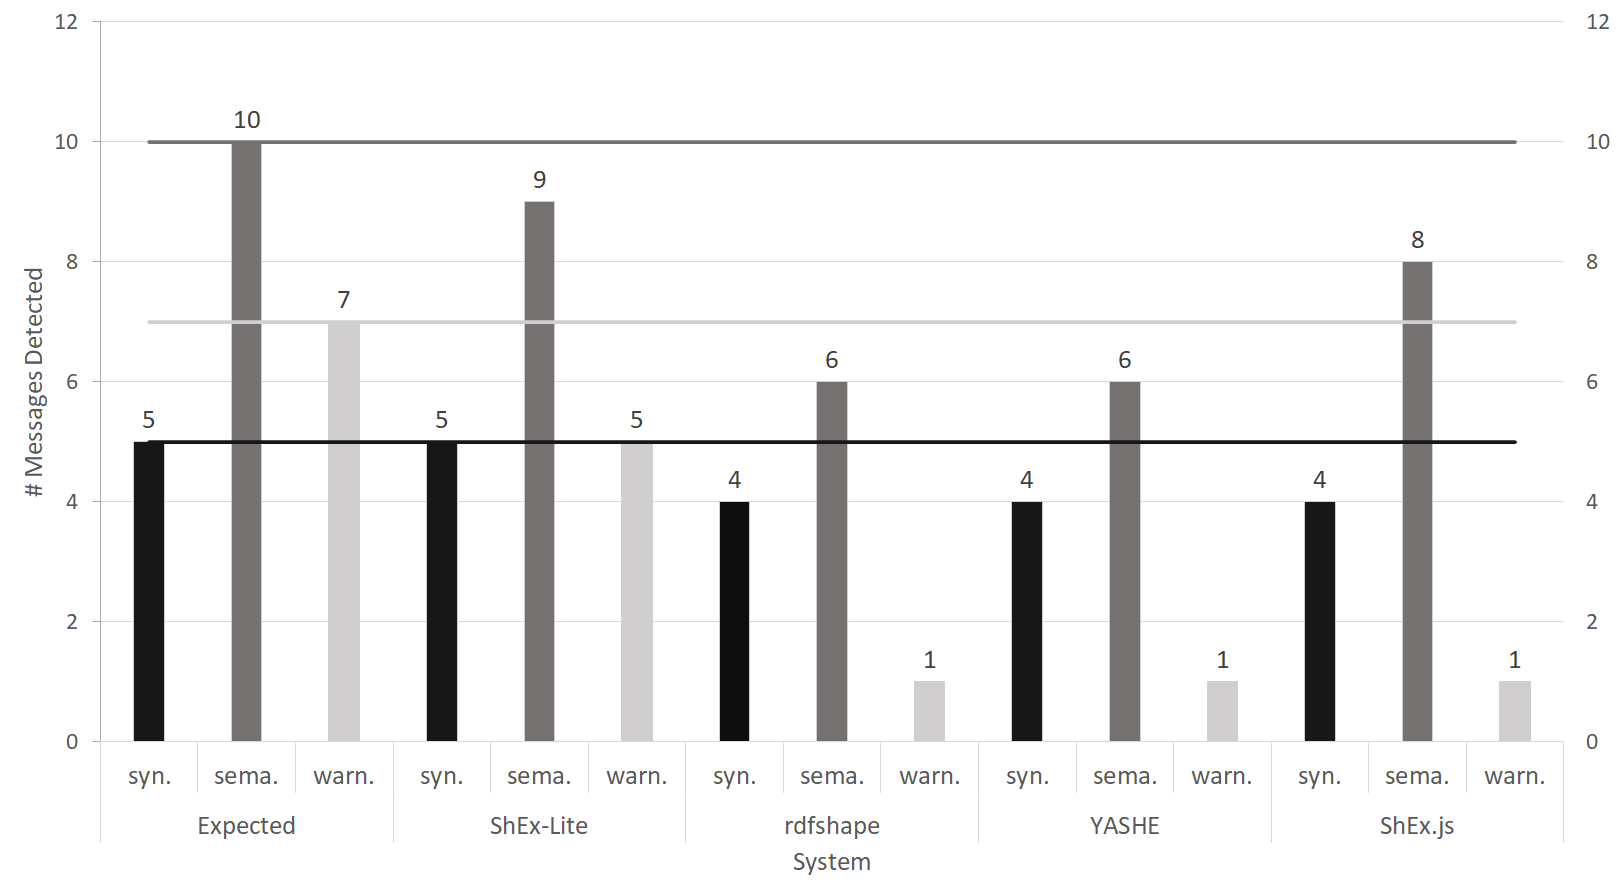
\includegraphics[width=\textwidth]{images/results-chart.png}
  \centering
  \caption[Bar chart for \cref{tb:errors-results}]{Bar chart for \cref{tb:errors-results}. Row 13 has been removed in order to normalize other results.}
  \label{fig:results-chart}
\end{figure}

From the results obtained and displayed, it can be
seen that ShEx-Lite is, together with ShEx.js, the
only system that detects multiple errors at the same
time. So systems like rdfshape, based on Shaclex, or
YASHE can benefit from the procedures proposed in this
work.

Another important observation is that when we have a syntactical error,
no system is capable of processing semantic errors or warnings that may
arise. This is completely normal since if the syntactic analysis phases
are not completed, the semantic analysis cannot be performed.

Regarding the second point of our methodology, \cref{tb:errors-q-results}
shows the results after evaluating the error messages (\cref{fig:err-non-def-pref-2,fig:err-non-def-pref-3,fig:err-non-def-pref-4})
produced by the different systems against the good practices defined in \cite{heeren2005top}.

\begin{figure}
  \begin{lstlisting}[numbers=left,basicstyle=\ttfamily\scriptsize]
error[E007]: prefix not defined
--> shape_with_error_cause_pref_not_defined.shex:17:3
  |
17| non_existing:label  xsd:string  +;
  | ^ the prefix `non_existing` has not been defined
  \end{lstlisting}
  \caption[Semantic error produced by ShEx-Lite for an undefined prefix]{Semantic error produced by ShEx-Lite for an undefined prefix.}
  \label{fig:err-non-def-pref-2}
\end{figure}

\begin{figure}
  \begin{lstlisting}[numbers=left,basicstyle=\ttfamily\scriptsize]
Prefix `non_existing` is not defined
  \end{lstlisting}
  \caption[Semantic error produced by RDFShape and YASHE for an undefined prefix]{Semantic error produced by RDFShape and YASHE for an undefined prefix.}
  \label{fig:err-non-def-pref-3}
\end{figure}

\begin{figure}[t]
  \begin{lstlisting}[numbers=left,basicstyle=\ttfamily\scriptsize]
error parsing input schema:
  Parse error; unknown prefix "non_existing"
  \end{lstlisting}
  \caption[Semantic error produced by RDFShape for an undefined prefix]{Semantic error produced by RDFShape for an undefined prefix.}
  \label{fig:err-non-def-pref-4}
\end{figure}

\begin{table}
  \centering
  \caption[Comparison of information provided in error and warning messages]{Comparison of information provided in error and warning messages.}
  \label{tb:errors-q-results}
  \resizebox{\textwidth}{!}{\begin{tabular}{c|c|c|c|c|c|c}
    & \begin{tabular}[c]{@{}c@{}}Source\\ File\end{tabular} & \begin{tabular}[c]{@{}c@{}}Line\\ Number\end{tabular} & \begin{tabular}[c]{@{}c@{}}Column\\ Number\end{tabular} & \begin{tabular}[c]{@{}c@{}}Code\\ Snipet\end{tabular} & \begin{tabular}[c]{@{}c@{}}Message\\ Title\end{tabular} & \begin{tabular}[c]{@{}c@{}}Message\\ Description\end{tabular} \\ \hline
ShEx-Lite & $\times$                                              & $\times$                                              & $\times$                                                & $\times$                                              & $\times$                                                & $\times$                                                      \\ \hline
RDFShape  &                                                       &                                                       &                                                         &                                                       & $\times$                                                &                                                               \\ \hline
YASHE     &                                                       &                                                       &                                                         &                                                       & $\times$                                                &                                                               \\ \hline
ShEx.js   &                                                       &                                                       &                                                         &                                                       & $\times$                                                &                                                              
\end{tabular}}
\end{table}

From the results, we interpret that all the existing tools, although they really
focus on data validation with Shape Expressions, would be greatly benefited
from using the methodologies described in this document.

Regarding the translation of schematics to object models, after executing the
translation on the dataset obtained from GitHub, the results found in \cref{tb:real-datase-results}
are extracted.

\begin{table}
  \centering
  \caption[Values obtained after compiling all the elements of our real case dataset with the ShEx-Lite system]{Values obtained after compiling all the
  elements of our real case dataset with the ShEx-Lite system. The dataset contains a total of 1.612 files of which only 19,4\%
  contain no errors and only 2,5\% contain neither errors nor warnings. Of the files without errors we were able to convert 29,4\%
  of the documents to domain model objects. While of those who had neither errors nor warnings, we were able to translate almost 50\%.}
  \label{tb:real-datase-results}
  \begin{tabular}{l|c|cc}
    ShEx Files       & 1.612 & 100\%                        &          \\ \cline{1-3}
    Without Errors   & 313   & 19.417\%                     &          \\ \cline{1-3}
    Without Warnings & 41    & 2.543\%                      &          \\ \cline{1-3}
    WE Transformed   & 92    & \multicolumn{1}{c|}{5.707\%} & 29.393\% \\ \hline
    WW Transformed   & 20    & \multicolumn{1}{c|}{1.241\%} & 48.780\%
  \end{tabular}
\end{table}

Of these values the first that strikes us is the large number of shapes that exist on GitHub
that have errors. This is explainable since we are only admitting a subset of the syntax.
Therefore we can consider these 313 as those shapes that are correct expressed in ShEx micro
Compact Syntax. However, of these 313 shapes that are in compact syntax, 86.9\% contain some
unused resource that generates warnings. On the one hand, this indicates that there is no system
that warns of these things and that almost 90\% of Shape Expressions users would benefit from the
analysis methods developed in this work.

Furthermore, our system is capable of translating almost 30\% of the schemas that do not have errors.
Of the shapes that do not contain any errors or warnings, our system translates almost 50\%. This tells
us that the more quality a shape has, the more likely it is to be compatible with object-oriented languages.